\documentclass[12pt,fleqn]{article}\usepackage{../common}
\usepackage[T1]{fontenc}
\begin{document}
Ders 23

Ak�� (Flux)

Aslinda ak�� cizgisel entegrallerin degisik bir seklidir. Diyelim ki $C$
egrisi ve $\vec{F}$ vektor alani var, o zaman $C$ uzerinden $\vec{F}$'in
ak���

\[ \int_C \vec{F} \cdot \hat{n} \ ds \]

olarak gosterilir. Simdi bu entegral icindeki ogelerin ne oldugunu tarif
edelim. 

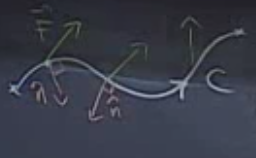
\includegraphics[height=3cm]{23_1.png}

$\hat{n}$ = $C$ egrisine dik olan birim normal vektordur, $\vec{T}$'ye 90
derece saat yonunde diktir. Saat yonunde dedik cunku mesela ustteki resimde
en soldaki $\hat{n}$ yukari da isaret ediyor olabilirdi, onu degil, asagi
dogru gideni sectik.

Entegral neyi hesaplar? Egri uzerindeki her noktada, vektor alani ile ayni
egrinin normalleri ile yapilan carpimlarin toplamini. Yani $C$'yi en ufak
parcalar $\Delta s$'lere ayirinca 

\[ Akis = \lim_{\Delta s \to 0} 
\bigg( \sum \vec{F} \cdot \hat{n} \ \Delta s \bigg) \]

Bu kavrami daha once hesapladigimiz ``yapilan i�'' karsilastirmak
gerekirse

\[ �� = \int_C \vec{F} \cdot d\vec{r} = \int_C \vec{F} \cdot \vec{T} \ ds \]

��i hesaplarken her noktada $\vec{F}$'in egri $C$'nin tegetine yansimasini
hesapliyorum. 

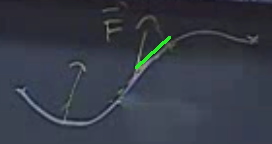
\includegraphics[height=2cm]{23_2.png}

Yani egri uzerinde hareket ederken ``$\vec{F}$ ile ne kadar birlikte, ne
kadar ona ters sekilde'' hareket edildiginin hesabini yapilan i� veriyor. 

Kiyasla ak�� hesabi, egri uzerinde hareket ederken $\vec{F}$'in egrinin
``ne kadar icinden gectiginin'' hesabi. Ruzgarli bir havada bir yolda
yuruyorum, ak�� ruzgarin bana ne kadar yandan carptigini gosteriyor. Akis
hesabi bu carpis saga dogru olunca onu pozitif, saga dogru olunca onu
negatif olarak hesaplar. 

Yani yapilan is $\vec{F}$'in tegetsel bilesenlerinin, yansimasinin toplami
ise, ak�� $\vec{F}$'in normal bilesenlerinin toplamidir. Bu ufak fark
haricinde bu iki hesap birbirinin aynisidir. Yani fiziksel anlamlari cok
farkli olabilir fakat matematiksel anlamda ikisi de bir cizgisel entegral,
ve hesaplanislari, tanimlari birbirine benzer. 

Anlatim baglaminda is hesabi icin $\vec{F}$'i bir kuvvet alani olarak gormek
anlatimi rahatlatiyor ($\vec{F}$ baska bir sey de olabilir). Ak��
baglaminda $\vec{F}$'i bir hiz alani (velocity field) olarak gormek
benzer bir rahatlik sagliyor. 

Bir siviyi dusunursek, ak�� birim zamanda $C$'nin icinden ne kadar sivinin
gectigini gosterir. Diyelim ki boyle bir alan alttaki gibi

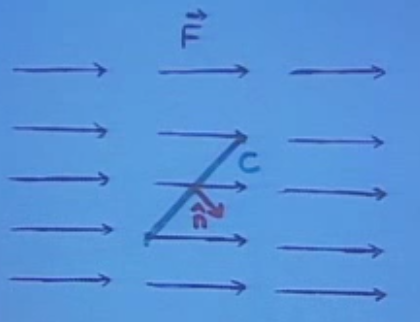
\includegraphics[height=4cm]{23_3.png}

Alan bir sabit alan, ama herhangi bir alana yeterince zoom edersek, o zaman
goruntusunun ustteki gibi olacagini dusunebiliriz. Simdi bu alan icinde
$C$'nin bir parcasi $\Delta s$'i hayal edelim, ve birim zaman icinde bu
alanin parcamiz icinden gecisini hayal edelim [hoca iki saydam ustuste
getirerek o parcayi oraya koydu, alanin gecisini gostermek icin parcayi
sola hareket ettiriyor, yani alanin saga dogru gecisini goruyoruz].

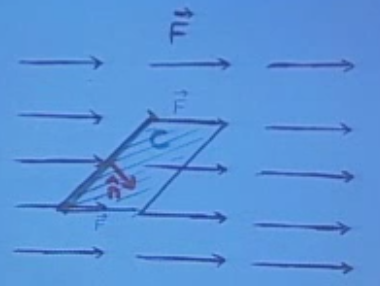
\includegraphics[height=4cm]{23_4.png}

Bu gecis birim zaman icinde ustteki gibi bir sekil olusturacaktir, bu
sekil bir paralelogramdir. Paralelogrami daha iyi gorebilmek icin ustteki
resmi alip 90 derece sola cevirelim, 

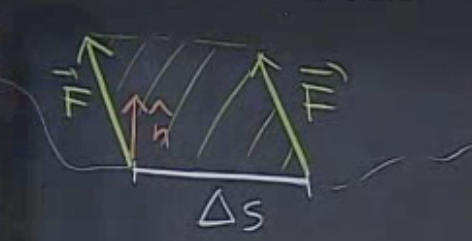
\includegraphics[height=3cm]{23_5.png}

Alan hesabi icin paralelogramin yuksekligi lazim, $\hat{n}$ bunun icin
gerekiyor. 

\[ Alan  = baz \cdot yukseklik \]

\[ = \Delta s \cdot (\vec{F} \cdot \hat{n} )\]

Tum bu hesaplari her parca icin toplarsak ak��� elde ederiz. 

Yaklasiksalligin bozulmamasi icin $\Delta s$'in oldukca kucuk olmasi, ve
zaman biriminin de ufak olmasi gerekir, mesela mikrosantim ile nanosaniye
gibi, yoksa $\vec{F}$ sabit bir alan olarak gorulemez. 

Ornek

$C$ orijinde oturan $a$ yaricapindaki, saat yonu tersinde bir cember egri. 

\[ \vec{F} = x\hat{i} + y\hat{j} \]

Geleneksel olarak saat yonu tersi, ve pozitif gecis saga dogru alindigi
icin bunun sonucu olarak alan kapali egriden ``disari'' cikmis olur. 

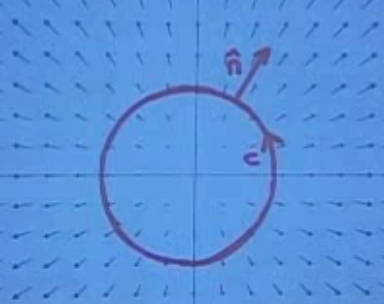
\includegraphics[height=5cm]{23_6.png}

Bir cemberde oldugum icin normal surekli cembere tam dik konumda, ve
$\vec{F}$'e surekli paralel. O zaman 

\[ \vec{F} \cdot \hat{n} = |\vec{F}||\hat{n}| \]

Fakat $\hat{n}$ birim vektor oldugu icin uzunlugu 1, o zaman

\[  = |\vec{F}| \]

Bu vektor alaninin buyuklugu nedir? Yani alanin her $x,y$ noktasindaki
vektorun buyuklugu (magnitude) nedir? Vektor buyuklugu karelerin toplaminin
karekokudur, $\sqrt{x^2 + y^2}$, ki bu buyukluk orijinden olan uzakliga
esittir. O zaman orijinde oturan cember uzerinde isek, uzaklik cemberin
yaricapina esittir, yani $a$. Yani ustteki formul soyle olur

\[ \vec{F} \cdot \hat{n} = |\vec{F}| = a\]

Cizgi entegrali bayagi kolay o zaman

\[ \int_C \vec{F} \cdot \hat{n} \ ds 
= \int_C a \ ds  = a \cdot \textit{C'nin uzunlugu}
\]

C'nin uzunlugu $2\pi a$ olduguna gore

\[ = 2\pi a^2 \]

Bu buyukluk beklenebilecegi uzere pozitif, cunku ak�� cemberden disari
dogru. 

Ornek

Ayni $C$ ama degisik $\vec{F}$ (bizim diger favori vektor alanimiz), 

\[ \vec{F} = <-y,x> \]

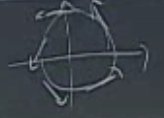
\includegraphics[height=2cm]{23_7.png}

Fakat burada vektorler her zaman cembere teget, o zaman o vektorlerin dik
bileseni olamaz, yani sifir olur. Burada ak�� olmadigini ciplak gozle bile
gorebiliyoruz. $\vec{F} \cdot \hat{n} = 0$, o zaman ak�� = 0. 

Tabii ki hesabi yapmak icin geometri her zaman yardim edemeyebilir, her
durumda isleyecek bir metot gerekli, aynen is hesabini yaptigimizda 
$Mdx +
Ndy$ hesabini yaptigimiz gibi. Ak�� hesabinda benzer bir yaklasim var. 

Bilesenleri Kullanarak Hesap

Hatirlarsak is hesabinda 

\[ d\vec{r} = \vec{T} \ ds = <dx,dy> \]

olmustu. O zaman dusunelim, ustte $\vec{T} ds$ kullandik, burada onun
yerine $\hat{n} \ ds$ var, onu nasil temsil edebiliriz? 

$\hat{n}$ aslinda $\vec{T}$'nin saat yonunde 90 derece dondurulmus hali
degil midir? O zaman 

\[ \hat{n}ds = <dy,-dx> \]

Donus saat yonunde oldugu icin eksi isaret $dx$ onunde. 

Demek ki $\vec{F} = <M,N>$ icin

\[ \int_C \vec{F} \cdot \hat{n} \ ds =
\int_C  <M,N> \cdot <dy,-dx> = 
\int_C -N dx + M dy
\]

Gerisi is hesabinda gordugumuz gibi. $x,y$ birbiriyle alakali, cogunlukla
ucuncu bir degisken $t$, $\theta$, vs gibi, ustteki formulu bu ortak
degisken cercevesinde tekrar yaziyoruz, sonra entegrali cozuyoruz. 

Peki Green'in Teorisi'nde yaptigimizi burada da yapabilir miyiz? Yani cizgi
entegralinin yerine bir cift entegral gecirmek. Cevap evet, ak�� hesabi
icin de isleyen Green Teorisi'nin bir versiyonu var. 

Ak�� Icin Green Teorisi

Eger $C$ bir $R$ alanini cevreliyorsa ve yonu saat yonu tersinde ise, ve
$\vec{F}=<P,Q>$ $R$ icinde her yerde turevi alinabilir ise, o zaman 

\[ \oint_C \vec{F} \cdot \hat{n} \ ds = 
\int \int_R div \ \vec{F} \ dA
\]

$div$ kelimesi uzaklasim (divergence) kavramindan geliyor ve formulu soyle:

\[ div \ <P,Q> = P_x + Q_y \]

Bu hesabi hatirlamak $curl$ formulunu hatirlamaktan daha basit aslinda,
$x,y$ uzerinden kismi turevler aliniyor ve bu turevler normal $P,Q$ sirasi
uzerinde uygulaniyor, sonuc toplaniyor. 

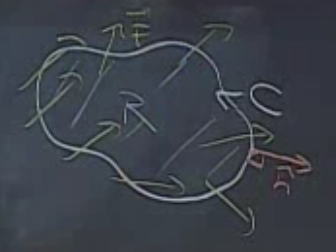
\includegraphics[height=4cm]{23_8.png}

Ak�� hesabi, o zaman, $C$ icinden gecerek $R$'den disari cikan ak��
hesabidir. Ustteki resimde mesela $C$'nin sag kismina etki eden $\vec{F}$
pozitif etki ederler, sol kismindakiler negatif olurlar (iceri giriyorlar)
ve bunlarin toplami tum ak��i verecektir. 

Bu formule ``normal formdaki Green Teorisi'' ismi de veriliyor. Is hesabi
icin olan anormal (!) oldugu icin degil tabii, sadece o form tegetsel,
buradaki normal. 

Ispat

Sunu ispat etmeye calisiyoruz

\[ \oint_C -Qdx + Pdy = \int \int_R (P_x + Q_y) dA 
\ \ \ \label{1}
\]

Bu formulu bir onceki derste kullandigimiz ispattaki forma indirgemeye
ugrasalim. Cebirsel olarak sol kismi soyle gorelim

\[ \oint_C 
\underbrace{-Q}_{M}dx + 
\underbrace{P}_{N}dy 
\]

Yani 

\[ M = -Q \]

\[ N = P \]

Onceki dersten biliyoruz ki 

\[ \oint_C Mdx + Ndy = \int \int_R (N_x - M_y) dA 
\ \ \ \label{2}
\]

Simdi (1) icindeki $P_x$ ve $Q_y$ nedir, onlari bulalim. 

\[ P_x = N_x \]

\[ Q_y = -M_y \]

Bunlari (1) icinde yerine koyarsak (2) formulunu elde ettigimizi
goruruz. Demek ki Green Teorisi'nin bu formu eskisi ile ilintili ve dogru. 

Ornek

Onceki ornek ile ayni vektor alani, ama bu sefer geometrik degil cebirsel
cozum kullanacagiz. 

\[ \vec{F} = x\hat{i} + y\hat{j} \]

Egri $C$ bir cember ve yaricapi $a$. 

Once $div \ \vec{F}$'i hesaplamak lazim. 

\[ div \ \vec{F}  = 
\frac{\partial }{\partial x}(x) + 
\frac{\partial }{\partial y}(y) = 
1 + 1 = 2 
 \]

\[ \oint_C \vec{F} \ \hat{n} ds = 
\int \int_R 2 dA = 
2 \int \int_R dA = 
2 \cdot \textit{R'nin alani}
 \]

\[ = 2\pi a^2 \]

Bu daha once buldugumuz sonuc ile ayni.

Peki ya $C$ orijinde degil baska bir yerde olsaydi? Mesela 

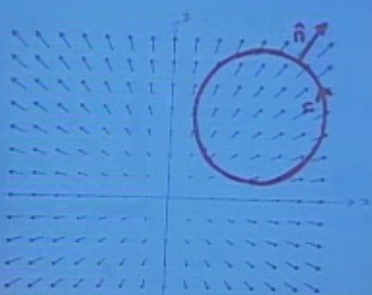
\includegraphics[height=4cm]{23_9.png}

Cizgi entegralini hesapladigimiz durumda bu cemberin parametrizasyonunu
bulup, o noktadaki vektor alani ile etkilesimini hesaplardik, vs. ve isler
uzardi. Ama Green'in Teorisine bakarsak orada cemberin merkezinin nerede
olduguyla alakali hicbir varsayim yok. O zaman $C$ nerede olursa olsun
sonuc her zaman $2\pi a^2$ cikacak. 

Simdi genel bir soruya gelelim. 

Uzaklasim yani $div$ neyi olcer? $curl$'un rotasyonel bir hesap yaptigini
biliyoruz. 

1) $div$ ak���n ne kadar ``yayildigini'', ``genisledigini'' olcer
diyebiliriz. Mesela cemberli ornekte her sey disari cikiyor, bir genisleme
var, $div$ pozitif. Eger ak�� tersine olsaydi (her sey iceri dogru) o zaman
$div$ negatif olurdu. 

2) Kaynak saglama orani, yani birim zamanda, birim alanda bir alandan,
mesela ne kadar sivinin dis sisteme ``ciktigi'', ``eklendigi''. Mesela
ustteki ornekte $div \ \vec{F} = 2$ demek, bu alandan dis sisteme surekli
sivi ekleniyor, sivi disari cikiyor anlamina gelir. 






\end{document}
